\section{Previous Work}

The Sensing Spaces project is an umbrella term for several problems related to air pollution in public spaces. Several students worked in different projects through the years, which inspired this project. Their work helped to develop this project, but the aim of this project is different from all previous work (Figure \ref{fig:venn_diagram}).
\begin{figure}[H]
    \centering
    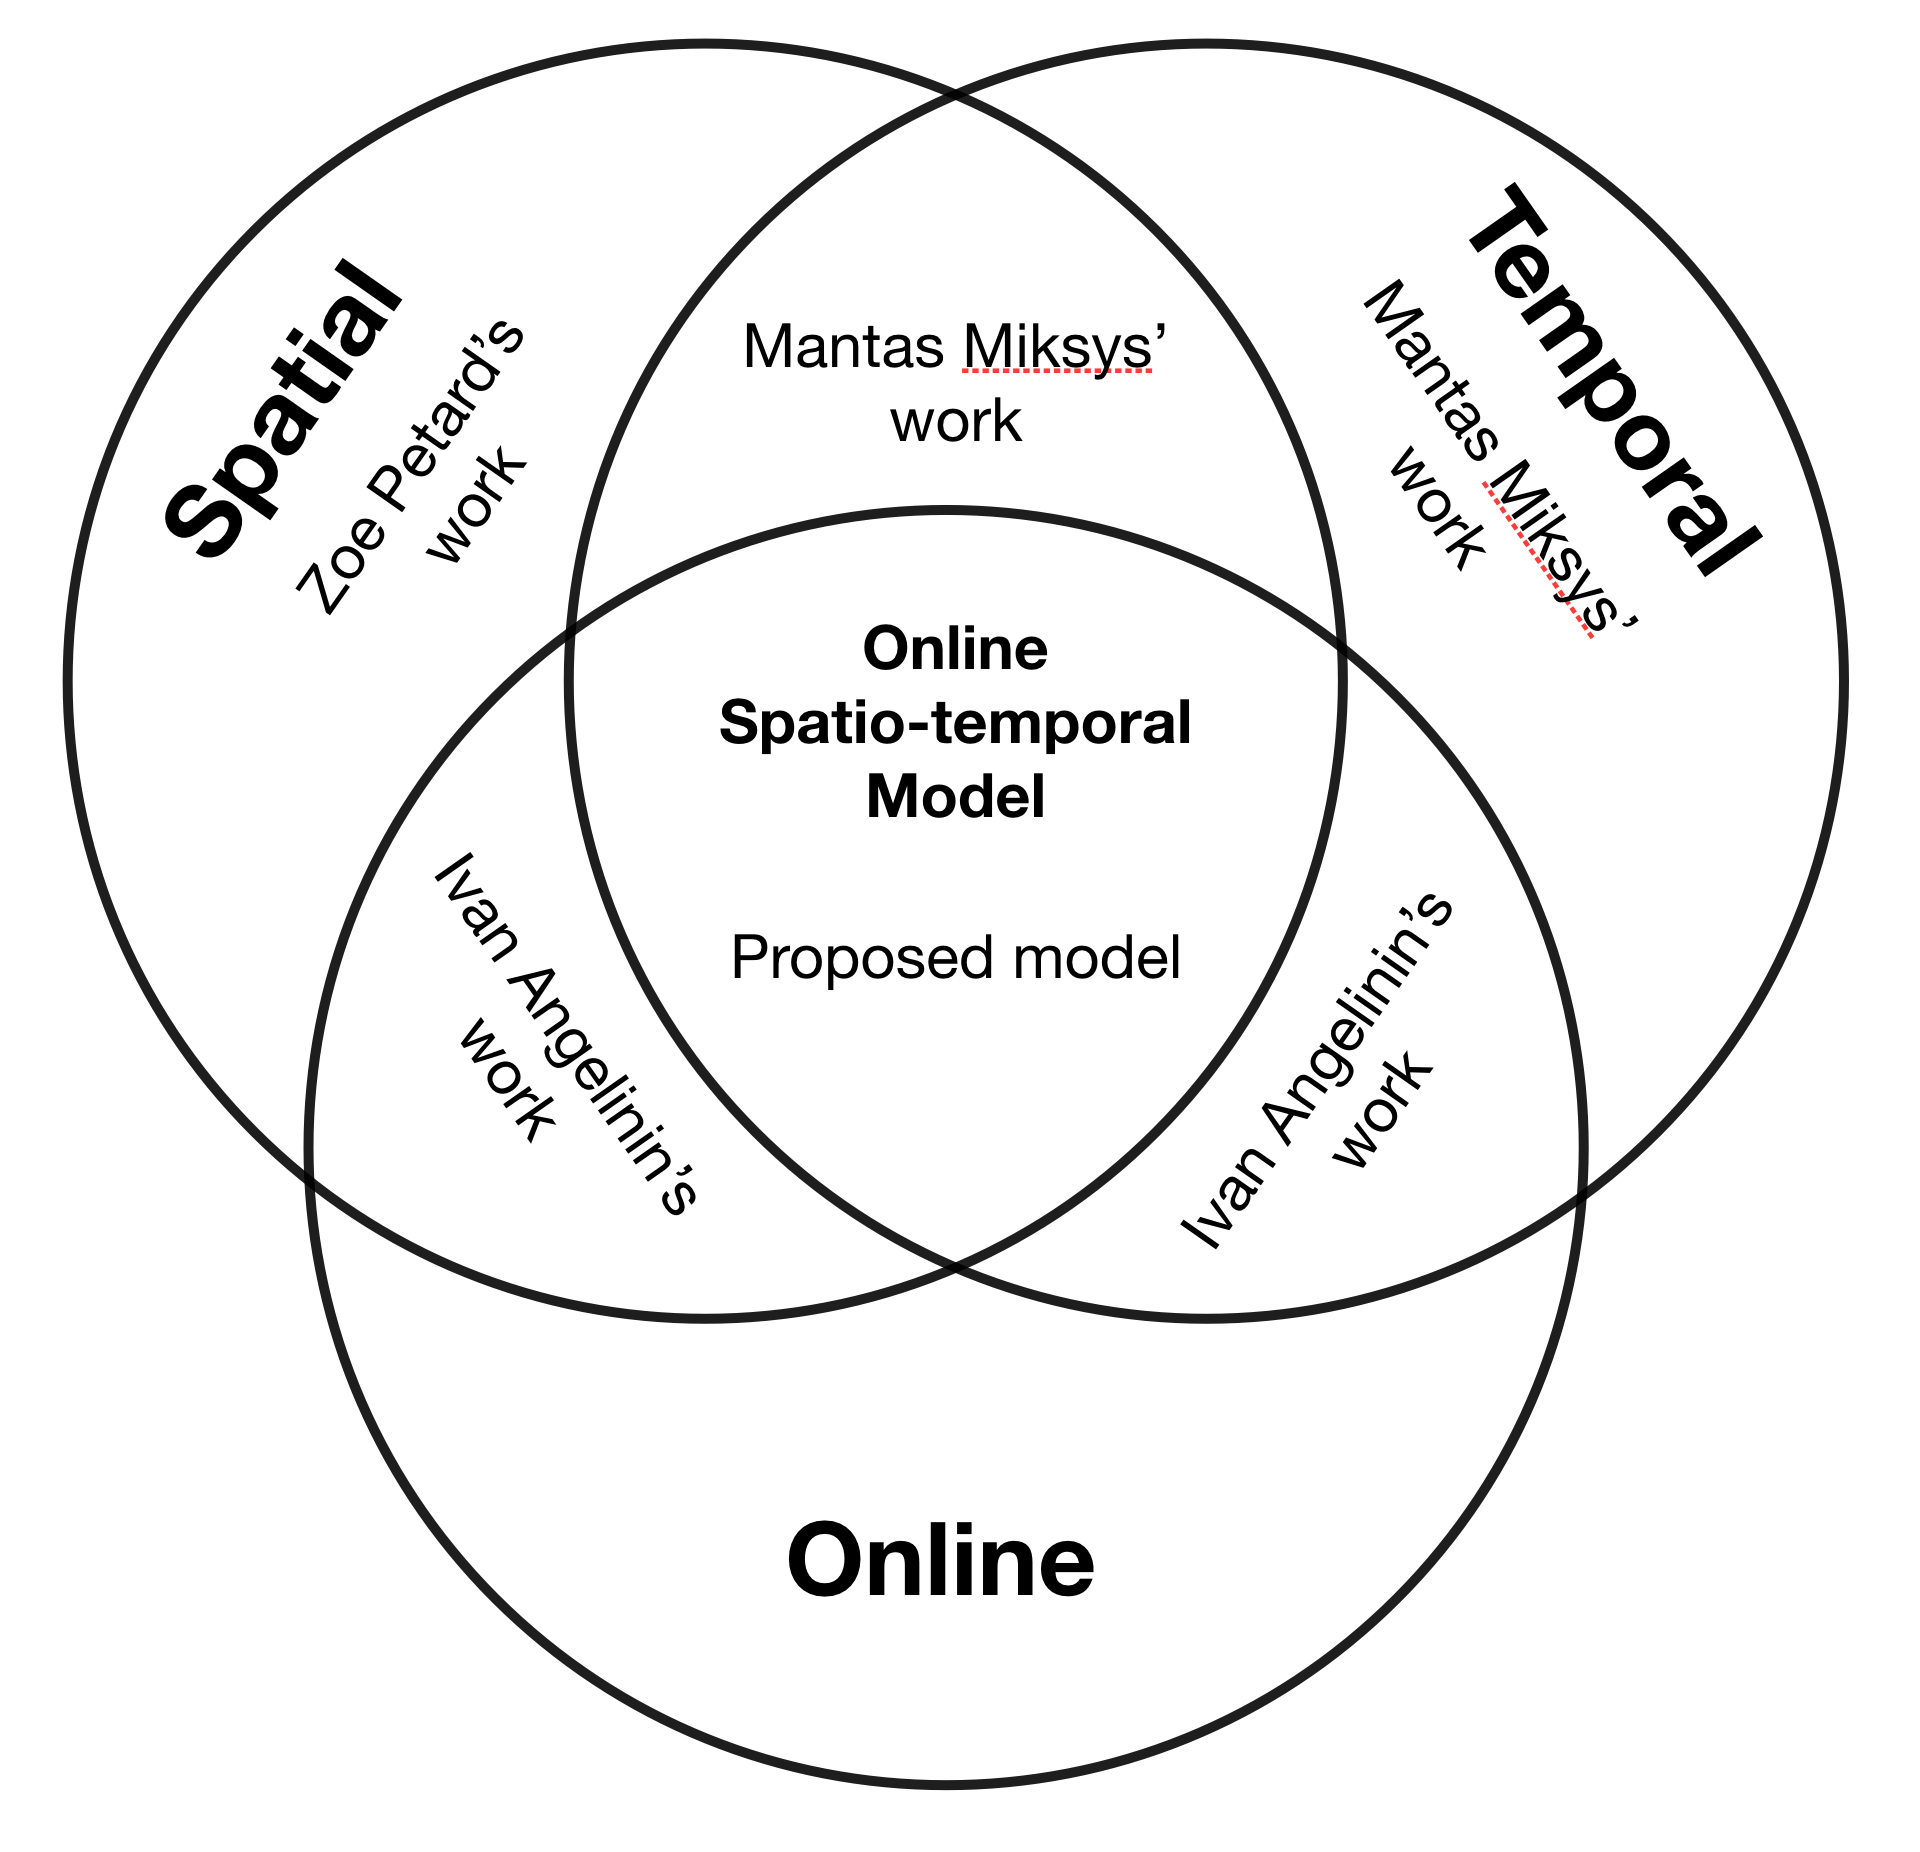
\includegraphics[width=.6\textwidth]{images/venn_diagram.png}
    \caption{Comparison of previous models}
    \label{fig:venn_diagram}
\end{figure}

%\subsection {Predicting Air Quality using Personal Exposure Monitors on Cyclists}
%This project was done by Aart Meijer in \hl{} and used 

\subsection {Predictions of PM2.5 and PM10 Concentrations Using Static and Mobile Sensors}

Mantas Miksys' 2016  project \cite{mantas} involved implementing and comparing offline temporal models and online spatial models using only static sensors for training and mobile sensors for validation. He also presented an offline spatio-temporal prediction model using only stationary sensors.  The models tested included Artificial Neural Networks, Decision Trees and others for temporal predictions and Inverse Distance Weighting, Kriging and Radial Basis Functions for spatial predictions. His work helped to define baselines and evaluation metrics for the model, and understand the temporal and spatial components of predictions.
The work presented differs in the way that this one is online, possible to implement for real-time application and can use mobile sensors' data collected in different time periods and different locations simultaneously with static sensor's data.

\subsection {Sensing Spaces: Improving Spatial and Temporal Prediction of Air Pollution Using Online Learning Algorithms}

Ivan Angelinin's 2018 project \cite{ivan} compared several approaches of online temporal models and online spatial models. He tested the following temporal models: Multilayer Perceptron, Linear Regression with Stochastic Gradient Descent, and Passive-Aggressive Regressor, and the following spatial models: Kriging and Radial Basis Functions. Although Angelinin's analysis of temporal and spatial models did not have any connection between themselves, it was instrumental in understanding how models performed and helped to choose models to use for the spatio-temporal model. Angelinin's code from the temporal and spatial model was not used, and code for this project was implemented from scratch using the same helper libraries that Ivan used in his work.


\subsection{Sensing Spaces: Planning journeys with least polluted, shortest routes in urban environments}
The work by Stefan Ivanov in 2018 \cite{stefan} consisted of making an application that performed route planning to find the least polluted route between a source and a destination on a map. This is an example of a potential application for the model presented in this report.

\subsection{Personal Exposure to Air Pollution with Different Modes of Transport and Urban Environments Using Wearable Sensors}

This project had a different scope. Mihai Visuian, in 2018, used mobile sensor data to classify urban environments and modes of transport using both supervised and unsupervised models\cite{mihai}.

\subsection{High Resolution Spatial Predictions of Air Pollution Levels in Edinburgh}
Zoë Petard \cite{zoe} developed the most recent work on the Sensing Spaces project. She implemented a convolutional neural network for spatial predictions of PM values using stationary data and validated on mobile data. She also collected data from stationary and mobile sensors throughout the project. Although this project is very different from what is proposed, her work was useful as the dataset and calibration factors were taken from this project for the model prediction experiments in this report.
\cite{zoe}




\section{Related Work}

\subsection{Online spatio-temporal models}

During the literature survey, no papers of an online spatio-temporal model for predicting air pollution levels were found. However, several applications of online spatio-temporal models were found for the most diverse applications: Hwa-Lung Yu \textit{et al.} produced an online spatio-temporal model to apply in epidemic dispersion of dengue fever in Taiwan. \cite{epidemic}, Gurkirt Singh \textit{et al.} applied and presented a solution for video frame prediction and action localisation. They stated in 2014 that in their field of study "current state-of-the-art approaches work offline, and are too slow to be useful in real-world settings" \cite{frame_pred}, , and for that reason, they published a paper that would allow for real-world settings. Lastly, a PhD thesis by Harold Soon Hong Soh entitled "Online spatio-temporal learning and prediction for adaptive robotic systems" \cite{robotics} focused on the robotics field, particularly tactile classification and learning assistance.

\subsection{Particulate matter concentration predictions}

Regarding air pollution predictions, the current state of the art is aligned with previous work performed in the Sensing Spaces project. Comparable work performed in Zurich \cite{zurich} shows an improvement in spatio-temporal models with a spatial resolution of $100 m \times 100 m$ and semi-daily temporal resolution using land-use and traffic characteristics. Both the work of Hasenfratz \textit{et al.} and this report aim at improving "detailed real-time pollution assessment" \cite{zurich}, and both used mobile data to make predictions: in Hasenfratz \textit{et al.} case with sensors installed in public buses. Their challenges such as "very sparse ground truth data", was a common problem in this project.

Huiping Peng's thesis \cite{peng} implemented, compared and evaluated the application of machine learning methods to air quality prediction using six stationary sensors in six different Canadian cities. Interestingly, this work included an online machine learning method entitled "Online Sequential Multiple Linear Regression" but the concept of using mobile sensors as additional data was not studied and predictions had a daily temporal scale of 24 hours.

Schneider \cite{low_cost} describes the use of low-cost sensors, a model that describes patterns of urban air pollution and data fusion techniques to make hourly predictions of nitrogen dioxide concentration in simulated data and real data in Oslo, Norway.

Another branch of machine learning, deep learning has been applied to air quality interpolation, prediction and feature analysis \cite{qi}. However, no reference of online learning or real-time application of deep learning was found in Qi's work of 2018. Spatio-temporal deep learning is also applied in the literature in other contexts such as traffic flow and high-frequency trading \cite{trading}.


Lastly, there are several model-based approaches to modelling pollution particles dispersion such as ADMS and AERMOD, developed in the United Kingdom, The Numerical Atmospheric-dispersion Modelling Environment (NAME), developed and used by the Met Office, RIMPUFF, a dispersion modelling system developed in Denmark, and CALPUFF, a meteorological and air quality modelling system produced in the United States of America. These are models that predict the dispersion of air pollutants, meteorological and air quality events in long-range events, especially compared to the PM predictions in this project.